\section{Bibliotecas de firmware}
O \textit{firmware} dos dispositivos foi desenvolvido no \textit{Framework Arduino}, que é uma abstração de códigos-fonte e bibliotecas comuns a diversas plataformas de \textit{\textit{hardware}}. Esta estrutura torna possível escrever programas para controlar uma ampla gama de placas microcontroladoras de Arduino e de outros fabricantes. O \textit{framework} fornece bibliotecas de código escritas em C/C++ para programação de microcontroladores e interação com dispositivos periféricos.

Para programar todas as funcionalidades do \textit{firmware} CLEAN, o código foi estruturado em um conjunto de classes em C++. Esta estrutura foi concebida visando sua reutilização em outras plataformas de microcontroladores e outros componentes de \textit{hardware} suportados no Framework Arduino (como ESP8266 da Espressif) e também para facilitar a revisão e manutenção do código. As classes desenvolvidas para o projeto estão distribuídas em quatro módulos principais, conforme mostrado na Figura \ref{fig:fw-libraries-structure}: o módulo \textit{Hardware Interfaces}, o módulo \textit{System Drivers}, o módulo \textit{}{Sensors} e o módulo \textit{Data}.

O módulo \textit{Hardware Interfaces} agrupa todas as classes e estruturas utilizadas para se comunicar com o \textit{hardware} periférico, como sensores, módulos de temporização, módulos de geolocalização e módulos de armazenamento. Os \textit{Drivers} implementam funcionalidades que podem ser utilizadas pelo programa principal independentemente do \textit{hardware} utilizado em cada dispositivo. O pacote \textit{Sensors} está no mesmo nível dos \textit{Drivers} e pode ser interpretado como um conjunto de \textit{drivers} especiais para os sensores, mas com a particularidade de ser específico para cada fabricante. Por fim, o pacote Dados engloba todas as funcionalidades relacionadas à preparação de dados de sensores para armazenamento e transmissão. Este pacote abstrai as informações de concentração adquiridas pelos sensores de gás a partir de detalhes específicos sobre o funcionamento e operação de seu \textit{hardware}.

\begin{figure}[h]
    \centering
    \caption{Conjunto de bibliotecas utilizadas para \textit{firmware} dos dispositivos CLEAN}
    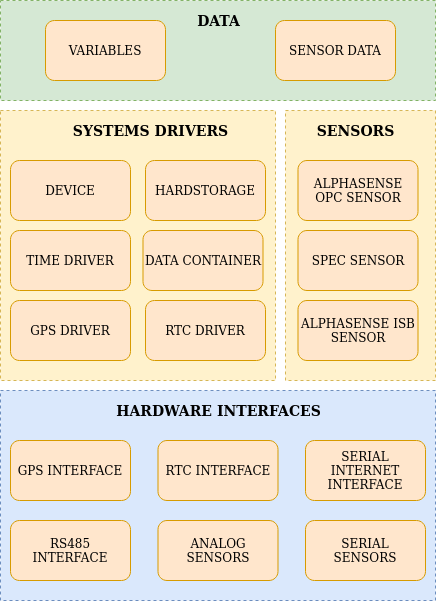
\includegraphics[width=0.75\linewidth]{chapters//2-CLEAN/Figuras/Diagrama de bibliotecas.png}
    \label{fig:fw-libraries-structure}
\end{figure}

\subsection{O módulo de interfaces de \textit{hardware}}

As Interfaces de \textit{Hardware} abrangem as funcionalidades relacionadas à comunicação e interface de sensores de gás, módulos de geoposicionamento (\acrshort{gps}) e relógio de tempo real (\acrshort{rtc}) que foram utilizados nos equipamentos desenvolvidos. O modo de operação e a saída dos sensores e de cada dispositivos de \textit{hardware} determinarão o seu esquema de conexão ao microcontrolador e a forma como sua leitura é implementada no \textit{firmware}.

A Figura \ref{fig:fw-libraries-hw-interfaces} mostra um diagrama das classes que foram implementadas para a versão atual do \textit{firmware}. As classes \texttt{SerialSensorInterface} e \texttt{AnalogSensorInterface} implementam interfaces para sensores digitais e analógicos, respectivamente. \texttt{SerialSensorInterface}, em particular, implementa uma interface para um sensor digital conectado através de um barramento \acrshort{uart} ou RS-485, por meio das classes filhas \texttt{UARTSensorInterface} e \texttt{RS485SensorInterface}. 

Cada classe implementa seu próprio método \texttt{sense()} que recebe como parâmetros um ponteiro para um objeto \texttt{Stream} (geralmente uma porta serial do microcontrolador), e um ponteiro para um \texttt{SerialParser}, que analisa as cadeias de caracteres com comandos ou dados enviados pelo sensor digital. O \texttt{SerialParser} é implementado numa camada superior pelas classes do módulo \texttt{Sensor}.

\begin{figure}[h]
    \centering
    \caption{Diagramas de classes do pacote \textit{Hardware} Interfaces}
    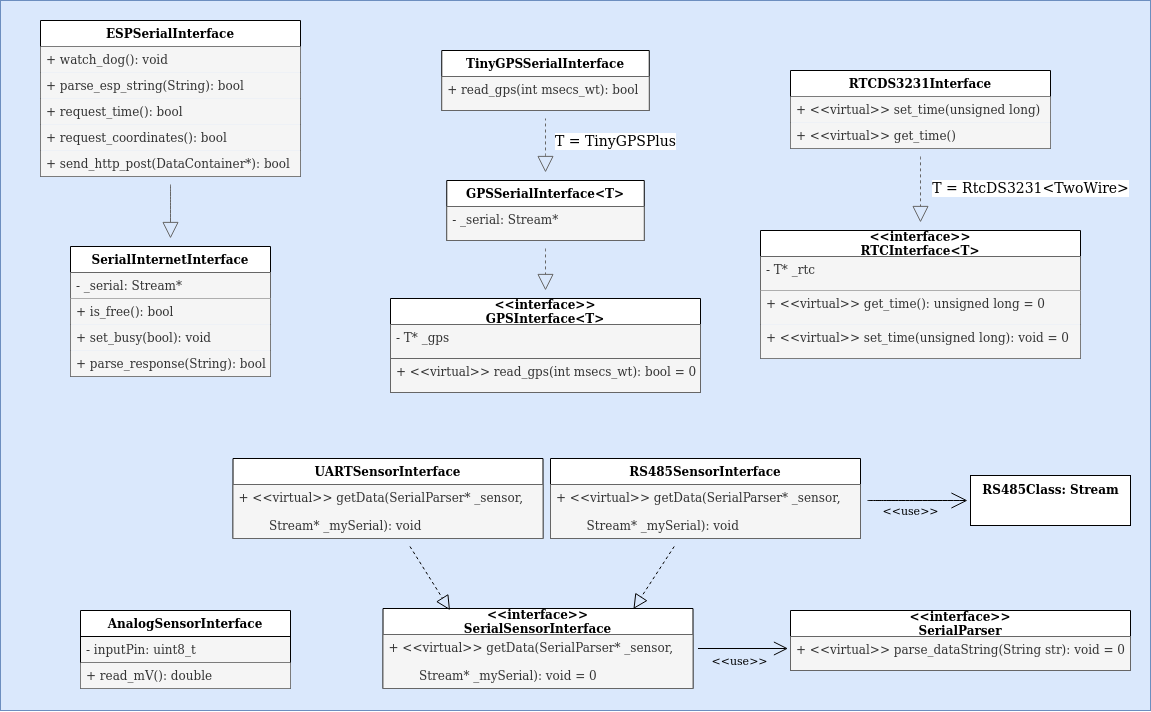
\includegraphics[width=0.90\linewidth]{chapters//2-CLEAN/Figuras/Diagrama-de-classes-Hardware-Interfaces.png}
    \label{fig:fw-libraries-hw-interfaces}
\end{figure}

A interface com um dispositivo serial para conexão à internet foi implementada através das classes \texttt{SerialInternetInterface} e \texttt{ESPSerialInterface}, esta última representando a conexão com o microcontrolador ESP8266. Foram criadas mais duas interfaces para módulos \acrshort{gps} e \acrshort{rtc}. Na versão atual do \texttt{firmware}, foram utilizadas as bibliotecas \texttt{TinyGPSPlus} e \texttt{RtcDS3221} para cada módulo respectivamente, porém, qualquer outra biblioteca ou módulo também pode ser usado, desde que seja criado como uma classe filha de \texttt{GPSSerialInterface} e \texttt{RTCInterface}. Para isso, as classes filhas deverão implementar os métodos virtuais: \texttt{readGPS()}, \texttt{set\_time()} e \texttt{get\_time()} respectivamente.

\subsection{O módulo \textit{drivers}}

Os \textit{Drivers} atuam como uma camada intermediária entre as Interfaces de \textit{Hardware} e o programa principal. Eles abstraem o \textit{hardware} dos dispositivos do código principal, permitindo sua reutilização independentemente dos módulos e bibliotecas utilizadas em um nível inferior. Alguns \textit{drivers} implementados para o \textit{firmware} foram:

\begin{itemize}
    \item O driver \texttt{HardStorage}, para armazenamento de dados em cartão \textit{SD}; 
    \item O \texttt{RTCDriver} para a Interface \acrshort{rtc};
    \item O \texttt{GPSDriver} para a Interface \acrshort{gps}; 
    \item O \texttt{TimeDriver} para gerenciamento das fontes de tempo no dispositivo, as quais podem provir de um módulo \acrshort{rtc}, um módulo \acrshort{gps} ou de um servidor \acrshort{ntp}
\end{itemize}

Esses quatro \textit{drivers} usam métodos estáticos, o que significa que podem ser usados sem necessidade de ter um objeto implementado no código. 

Os outros dois \textit{drivers} que foram implementados estão relacionados ao tratamento dos dados. São eles o \texttt{DataContainer} e o \texttt{Smoother}. A Figura \ref{fig:fw-libraries-drivers} mostra o diagrama de classes deste módulo. A continuação são resumidos alguns dos principais métodos e atributos de cada uma das classes pertencentes ao módulo \texttt{Drivers}.

\begin{figure}[h]
    \centering
    \caption{Diagrama de classes do Módulo \textit{Drivers}}
    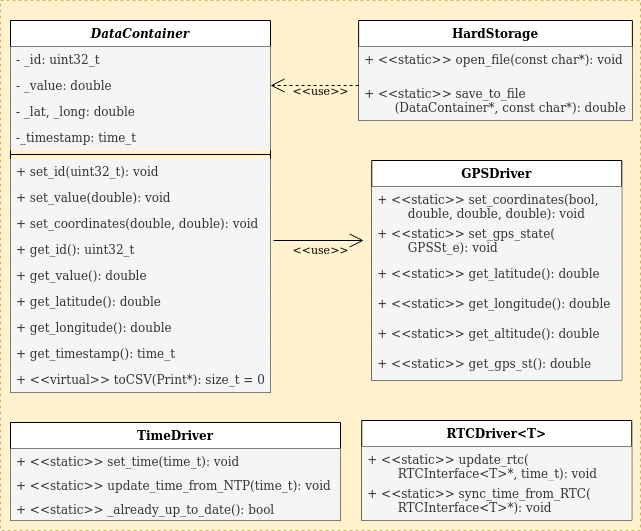
\includegraphics[width=0.90\linewidth]{chapters//2-CLEAN/Figuras/Diagrama-de-classes-System-Drivers-1.png}
    \label{fig:fw-libraries-drivers}
\end{figure}

\subsubsection{TimeDriver}
Esta classe registra a data e hora internas do sistema e fornece métodos para retornar informações de data e hora em diferentes formatos. O método \texttt{set\_time(time\_t)} define a data e hora do sistema. Internamente, ele invoca o método \texttt{setTime()} da biblioteca \texttt{Time.h} do framework Arduino. Recebe como parâmetro um número inteiro de 32 bits contendo a data e hora fornecidas por alguma fonte de relógio externa (um módulo \acrshort{gps}, um módulo \texttt{rtc} ou um servidor \texttt{ntp}).
\subsubsection{GPSDriver}
Esta classe controla a interface com um módulo \texttt{gps}, armazena as informações das coordenadas geográficas do sistema e fornece métodos para acessá-las, sendo eles:

\begin{itemize}
    \item \texttt{{static} get\_latitude(): double}
    \item \texttt{{static} get\_longitude(): double}
    \item \texttt{{static} get\_altitude(): double}
    \item \texttt{{static} get\_gps\_st(): GPSSt\_e}
\end{itemize}

Esses métodos fornecem as informações de geolocalização armazenadas no \texttt{GPSDriver}, bem como o estado dessas informações. As informações de geolocalização podem estar OK ou desatualizadas. Esses dois valores são retornados como uma enumeração do tipo \texttt{GPSSt\_e}.

Outros dois métodos definem as coordenadas geográficas do sistema e o estado dessa informação. Esses métodos são chamados por uma instância de GPSInterface. Eles são:

\begin{itemize}
    \item \texttt{{static} set\_coordinates(): void}
    \item \texttt{{static} set\_gps\_state(): void}
\end{itemize}

\subsubsection{RTCDriver}
Esta classe controla a interface com um módulo \acrshort{rtc}. O método \texttt{update\_rtc(RTCInterface*, time\_t)} é chamado sempre que o módulo \acrshort{rtc} precisa ser atualizado. Recebe como parâmetro um ponteiro para a instância do \texttt{RTCInterface} que será atualizada e a data e hora. O método \texttt{sync\_time\_from\_RTC(RTCInterface*)} retorna a data e hora a partir do ponteiro ao tipo \texttt{RTCInterface} passado como parâmetro

\subsubsection{DataContainer}
Esta é uma classe abstrata que contém informações sobre a leitura de uma variável. Essas informações são: o identificador da variável que está sendo medida e o valor dessa variável; as coordenadas; e a data e hora onde a valor foi medido. Objetos desta classe são usados para armazenar dados no cartão SD e para enviar postagens \textit{HTTP}. O método \texttt{toCSV(Print*)} é um método virtual puro para formatar os dados de uma leitura de variável e armazená-los em um arquivo \acrshort{csv}. Por se tratar de um método virtual, ele deve ser implementado pelas classes filhas de \texttt{DataContainer}. Desta forma cada aplicação pode ter seu próprio formato de armazenamento das informações.

\subsubsection{HardStorage}
Esta classe contém os métodos para leitura e gravação de e para um cartão SD. Para leitura, o método \texttt{open\_file(const char*)} abre o arquivo no qual as operações de leitura/gravação serão executadas. O método recebe o nome do arquivo como parâmetro. Já para a escrita no cartão, o método \texttt{save\_to\_file<T>(DataContainer*, const char*)} grava dados em um arquivo no cartão SD. O nome do arquivo é passado como parâmetro, juntamente com os dados a serem salvos. A função espera um ponteiro para um \texttt{DataContainer}, que na versão atual do \textit{firmware} são objetos do tipo \texttt{SensorData}. O objeto \texttt{SensorData} implementa o método \texttt{toCSV(Print*)}, que recebe um ponteiro para o arquivo e armazena os dados nele.

\subsection{O módulo Sensores}

As classes deste pacote encapsulam a lógica de leitura de cada sensor, considerando as especificações de cada fabricante. Eles fazem uso das interfaces de sensores implementadas no pacote de Interfaces de \textit{Hardware}. Dois fabricantes de sensores foram utilizados no \textit{hardware} dos equipamentos desenvolvidos no contexto deste trabalho: Alphasense e SPEC Sensors. As interfaces dos sensores Alphasense e SPEC diferem na forma como foram implementadas. As saídas dos sensores Alphasense são dois sinais de tensão analógicos. Os sensores SPEC, por outro lado, fornecem os valores de concentração de gás, temperatura e umidade em uma cadeia de caracteres que é enviada através de uma interface \acrshort{uart}. A Figura \ref{fig:fw-libraries-sensors} mostra um diagrama das classes implementadas para este módulo.

\begin{figure}[h]
    \centering
    \caption{Diagramas de classes do módulo Sensors}
    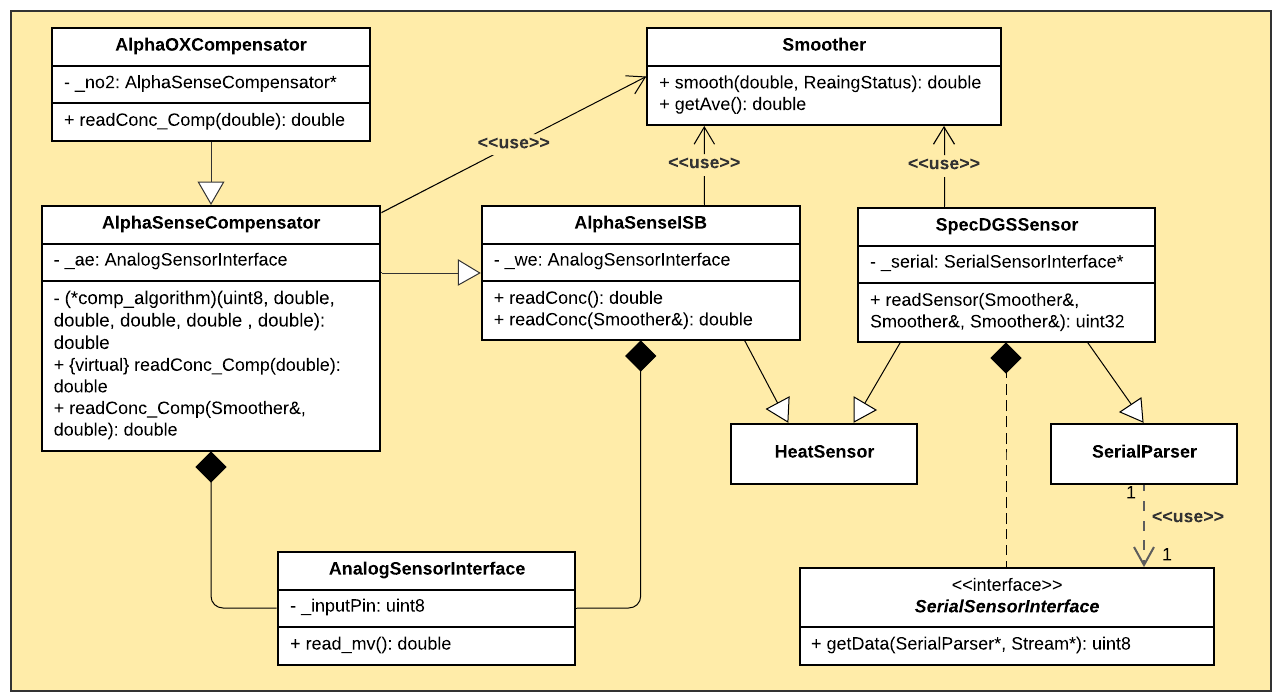
\includegraphics[width=0.90\linewidth]{chapters//2-CLEAN/Figuras/Diagrama-de-classes-Sensors-Package.png}
    \label{fig:fw-libraries-sensors}
\end{figure}

A base para o interfaceamento dos sensores Alphasense é a leitura de duas entradas analógicas do microcontrolador utilizando a função \texttt{analogRead()} do \textit{framework} Arduino. Por esse motivo, a classe base para modelagem dos sensores Alphasense é a classe \texttt{AnalogSensorInterface}. Ela representa uma entrada analógica identificada pelo atributo \texttt{\_inputPin}, e seu método \texttt{read\_mv()} converte o valor digital adquirido pelo conversor analógico-digital do Arduino, em um valor de tensão entre 0 – 5 V. Este método pode receber como parâmetro uma referência a um objeto do tipo \texttt{Smoother}, que por sua vez deve estar associado a um objeto \texttt{Variable}. Assim, são vinculadas as variáveis físicas modeladas no \textit{firmware} com a respectiva interface de \textit{hardware}; neste caso uma entrada analógica.

A classe \texttt{HeatSensor} representa um sensor que precisa de um tempo de aquecimento para funcionar. A lógica que determina a validade das leituras dos sensores é implementada dentro desta classe, levando em consideração um período de aquecimento para cada sensor. Do \texttt{HeatSensor} derivam as classes que representam os sensores Alphasense e SPEC, uma vez que ambos são sensores eletroquímicos amperométricos que requerem um intervalo de aquecimento para garantir que as leituras sejam válidas. A continuação resumem-se as principais propriedades das classes relacionadas ao interfaceamento dos sensores de gases.

\subsubsection{\texttt{AlphaSenseISB}}
Esta classe representa um sensor Alphasense com um circuito de condicionamento do tipo \acrshort{isb}. O sufixo "ISB" indica que o circuito de condicionamento usado é a placa de detecção individual do fabricante do sensor. Esta classe não incorpora nenhum algoritmo de compensação.

\textbf{Atributos:}
\texttt{\_we: AnalogSensorInterface}: Este é um atributo privado que representa a entrada analógica conectada ao eletrodo de trabalho (WE) do sensor

\textbf{Métodos:}
\texttt{readConc(): double}
\texttt{readConc(Smoother\&): double}
Estes são métodos públicos que convertem o valor de tensão lido pelo atributo \texttt{\_we} em um valor de concentração, levando em consideração a sensibilidade do sensor informada pelo fabricante. A referência ao objeto \texttt{Smoother} associa o sensor à variável física correspondente e retorna um valor suave das leituras da variável.

\subsubsection{\texttt{AlphaSenseCompensator}}
Derivado do \texttt{AlphaSenseISB}, representa um sensor Alphasense com um algoritmo de compensação. Os sensores da série Alphasense B4 podem usar diferentes algoritmos de compensação dependendo do gás ao qual são sensíveis. Por isso, cada algoritmo é inerente a cada objeto e não à classe

\textbf{Atributos:}
\texttt{\_ae: AnalogSensorInterface}: Este é um atributo privado que representa a saída do eletrodo auxiliar (AE) do sensor eletroquímico. O valor de saída deste eletrodo é usado nos algoritmos de compensação.

\textbf{Métodos:}
\texttt{(*comp\_algorithm)(uint8, double, double, double, double, double): double}: Este é um ponteiro para a função que implementa o algoritmo de compensação. As funções recebem como parâmetros as variáveis necessárias para o cálculo do algoritmo, dentre eles a temperatura.

\texttt{{virtual} readConc\_Comp(double): double}
\texttt{readConc\_Comp(Smoother\&, double): double}
Estes são métodos públicos que leem os valores de tensão armazenados nos atributos \texttt{\_we} (herdados do \texttt{AlphaSenseISB}) e \texttt{\_ae}. Eles aplicam o algoritmo de compensação correspondente e retornam um valor de concentração. Ambos os métodos recebem como parâmetros a temperatura ambiente e uma referência a um objeto \texttt{Smoother}, como no \texttt{AlphaSenseISB}.

\subsubsection{\texttt{AlphaOXCompensator}}
Este é um caso especial para sensores de ozônio que utilizam um algoritmo de compensação. Os sensores de ozônio medem, na verdade, a soma das concentrações de ozônio e dióxido de nitrogênio, portanto, o valor da concentração de dióxido de nitrogênio é exigido pelo algoritmo de compensação.

\textbf{Atributos:}
\texttt{\_no2: AlphaSenseCompensator*}: Para acessar o sensor de dióxido de nitrogênio, a classe \texttt{AlphaOXCompensator} usa um ponteiro para um objeto \texttt{AlphaSenseCompensator} que representa o sensor de dióxido de nitrogênio.

\textbf{Métodos:}
\texttt{readConc\_Comp(double): double}: Este método lê o valor da concentração do sensor de ozônio e aplica um algoritmo de compensação considerando também a concentração de dióxido de nitrogênio. Para vincular essas leituras a um objeto do tipo \texttt{Variable}, a classe \texttt{AlphaOXCompensator} utiliza o mesmo método \texttt{readConc\_Comp()} herdado da classe \texttt{AlphaSenseCompensator}, que recebe uma referência a um objeto do tipo \texttt{Smoother}.

\subsubsection{Interface com sensores seriais}

A interface com os sensores SPEC é realizada através da classe abstrata \texttt{SerialSensorInterface}. Esta classe fornece métodos para a leitura dos sensores através da porta serial do microcontrolador. A comunicação entre os sensores e o Arduino pode ser implementada através de uma interface \acrshort{uart} ou através de um barramento RS-485. Ambas as interfaces de comunicação são modeladas nas classes \texttt{UARTSensorInterface} e \texttt{RS485SensorInterface}, que derivam de \texttt{SerialSensorInterface}.

A classe \texttt{specDGS\_sensor} funciona como uma camada intermediária entre a interface de \textit{hardware} e as classes do módulo \texttt{Data}. Por representar um sensor eletroquímico que necessita de um período de aquecimento, esta classe também herda da classe \texttt{HeatSensor}. As instâncias de \texttt{specDGS\_sensor} têm a finalidade de ler e analisar as cadeias de caracteres enviadas pelos sensores SPEC, com as medições de temperatura, umidade e concentração de gás. Esta classe também é responsável por validar as medições levando em consideração o tempo de aquecimento dos sensores e possíveis erros na comunicação serial. O método \texttt{readSensor()} lê os valores de concentração, temperatura e umidade e os disponibiliza aos objetos de tipo \texttt{Variable} correspondentes por meio das referências \texttt{Smoother} que recebe como parâmetros.

O atributo \texttt{\_serial} da classe \texttt{specDGS\_sensor} é um ponteiro para um objeto do tipo \texttt{SerialSensorInterface}, que é atribuído durante a construção de cada instância \texttt{specDGS\_sensor}. O ponteiro pode ser um objeto do tipo \texttt{UARTSensorInterface} ou \texttt{RS485SensorInterface}, dependendo apenas da interface de comunicação implementada no \textit{hardware}. Os objetos \texttt{specDGS\_sensor} representam os sensores SPEC, e as instâncias derivadas da classe abstrata \texttt{SerialSensorInterface} representam a interface com esses sensores, que no \textit{hardware} é uma única porta serial.

\subsection{O módulo \texttt{Data}}

A Figura \ref{fig:fw-libraries-data} mostra o diagrama de classes do módulo \texttt{Data}. Como já mencionado, este módulo funciona como uma camada intermediária que prepara e formata as medições obtidas no \textit{hardware} do sensor para seu armazenamento e transmissão. É formado por duas classes principais: \texttt{Variable} e \texttt{SensorData}.

A classe \texttt{SensorData} método prepara os dados para transmissão remota e armazenamento local. Cada objeto do \texttt{SensorData} está associado a um único objeto do tipo \texttt{Variable}, que representa uma variável física com um identificador único. Vale ressaltar que, embora no \textit{firmware} cada variável física seja representada por um único identificador, no \textit{hardware} uma ou mais dessas variáveis podem estar vinculadas a um mesmo transdutor. O número de identificação que representa cada variável física é o que associa cada objeto da classe \texttt{Variable} ao objeto do tipo \texttt{SensorData} correspondente. Este número é armazenado em cada classe nos atributos \texttt{\_sensorID} e \texttt{\_id} como valores inteiros de 32 bits.

\begin{figure}[h]
    \centering
    \caption{Diagrama de classes do pacote \texttt{Data}}
    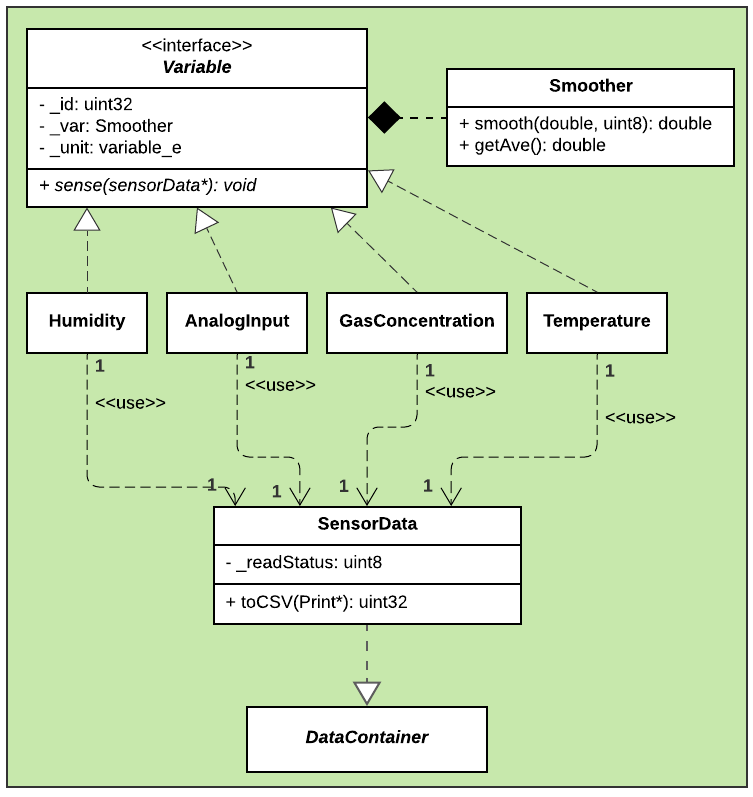
\includegraphics[width=0.80\linewidth]{chapters//2-CLEAN/Figuras/Diagrama-de-classes-Data-Package.png}
    \label{fig:fw-libraries-data}
\end{figure}

Objetos do tipo \texttt{SensorData} contêm o valor das variáveis físicas às quais estão associados, juntamente com informações sobre a data, hora e local onde as medições foram feitas. O valor de cada variável é armazenado no atributo \texttt{\_value}, o qual pode ser um dado bruto medido em determinado instante de tempo ou uma média de valores adquiridos durante uma janela temporal. O método \texttt{toCSV()} consolida e prepara as informações do valor medido pelo sensor, sua geolocalização, e a data e hora em que a medição foi realizada, no formato \acrshort{csv}.

A classe \texttt{Variable} atua como uma camada intermediária entre a camada de \textit{hardware} do sensor e a classe \texttt{SensorData}. Os objetos desta classe representam as variáveis físicas que estão sendo monitoradas, porém, não contêm suas quantidades, pois esses valores estão armazenados em objetos do tipo \texttt{SensorData}. Como já mencionado, o atributo \texttt{\_id} contém o identificador da variável física que representa. O atributo \texttt{\_unit} representa a unidade de medida da variável física que está sendo monitorada. O atributo \texttt{\_var}, do tipo \texttt{Smoother}, funciona como um buffer de memória no qual os objetos que implementam a interface de \textit{hardware} dos sensores podem colocar as amostras da variável medida. Desse mesmo buffer, o objeto \texttt{SensorData} associado pode extrair o valor médio das amostras. O número de amostras de cada buffer depende da capacidade que for programada. Os diagramas nas Figuras \ref{fig:fw-read-write-smoother} e\ref{fig:fw-sense-seq} ilustram este processo.

\begin{figure}[t]
    \centering
    \caption{Processo de leitura de uma variável}
    \begin{subfigure}{0.495\textwidth}
        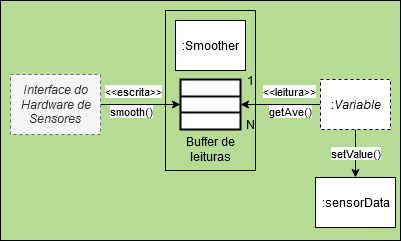
\includegraphics[width=\textwidth]{chapters/2-CLEAN/Figuras/Diagrama R_W Buffer Smoother.png}
        \caption{Processo de escrita e leitura no buffer da classe \textit{Smoother}}
        \label{fig:fw-read-write-smoother}
    \end{subfigure}
    \hfill
    \begin{subfigure}{0.495\textwidth}
        \includegraphics[width=\textwidth]{chapters/2-CLEAN/Figuras/Diagramas de sequências.png}
        \caption{Diagrama de sequências do método \textit{sense()}}
        \label{fig:fw-sense-seq}
    \end{subfigure}
    \hfill
    \label{fig:fw-read-variable}
    \fonte{Desenvolvido pelo autor (2023)}
\end{figure}

Os objetos que representam os sensores, gravam as leituras de cada variável física no buffer de amostragem através do método \texttt{smooth()} da classe \texttt{Smoother} (\ref{fig:fw-read-write-smoother}). Já a classe \texttt{Variable} acessa a média das amostras invocando o método \texttt{getAve()} do atributo \texttt{\_var}. Esse valor médio é transferido para o objeto \texttt{SensorData} associado por meio do método \texttt{setValue()}. O processo de leitura e transferência do valor médio das amostras para o objeto \texttt{SensorData} acontece dentro do método \texttt{sense()} definido na classe \texttt{Variable}. A Figura \ref{fig:fw-sense-seq} mostra o diagrama de sequência para este método.

A função \texttt{sense()} é um método virtual puro, portanto, as instâncias que derivam da classe abstrata \texttt{Variable} devem implementá-la. A sequência principal de ações executadas pelo método é comum a todas as classes derivadas. Quando o método \texttt{sense()} é invocado, a classe filha de \texttt{Variable} acessa, através do método \texttt{getAve()} de \texttt{Smoother}, o valor médio das amostras. Este valor é então passado para o objeto do tipo \texttt{SensorData} associado através do método \texttt{setValue()}. O objeto do tipo \texttt{SensorData}, por sua parte, armazena a data, a hora e o local onde foi feita a medição, bem como o status da leitura (método \texttt{getReadSt()}).

Os tipos de variáveis físicas implementadas na versão atual do \textit{firmware} foram: Temperatura, Umidade, Concentração de gás e Entrada Analógica. Esta última representa uma tensão analógica que pode ser lida como um sinal de tensão entre 0 – 5 V. Essas variáveis foram modeladas em classes filhas de \texttt{Variable} como \texttt{Temperature}, \texttt{Humidity}, \texttt{GasConcentration} e \texttt{AnalogInput}. Por serem classes filhas, todas possuem os mesmos atributos de \texttt{Variable}, mas cada uma implementa seu próprio método \texttt{sense()}.